\documentclass[a4paper,12pt]{article}
\usepackage[T2A]{fontenc}
\usepackage[utf8]{inputenc}
\usepackage[english,russian]{babel}
\usepackage[margin=2cm]{geometry}
\usepackage{fancyvrb}
\usepackage{inconsolata}
\usepackage{graphicx}

\newcommand\userinput[1]{\textbf{#1}}

\newcounter{problemnumber}

\newenvironment{problem}[1]
	{\addtocounter{problemnumber}{1}\arabic{problemnumber}. (#1)}
	{\vspace{6pt}}

\title{Домашняя работа 24}
\date{}
\begin{document}
\maketitle{}

\emph{Во всех программах размер экрана $640 \times 480$. Эти числа должны
    задаваться в виде констант в начале программы.}

\begin{problem}{Культин, 201}
    Написать программу, которая выводит на экран контур пятиконечной звезды,
    как показано на рис.~\ref{fig:star}.
\end{problem}

\begin{problem}{Культин, 203}
    Написать программу, которая вычерчивает на экране шестиугольник.
\end{problem}

\begin{problem}{Культин, 207}
    Написать программу, которая вычерчивает на экране узор, изображённый на
    рис.~\ref{fig:kultin207}.
\end{problem}

\begin{problem}{Культин, 208}
    Написать программу, которая выводит на экран концентрические окружности
    (окружности разного диаметра, но с общим центром). Окружности должны быть
    разного цвета.
\end{problem}

\begin{figure}
\centering
\begin{minipage}{.5\textwidth}
  \centering
  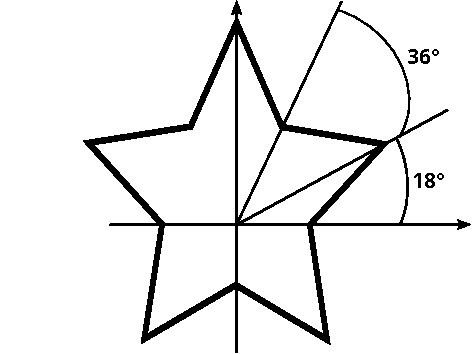
\includegraphics{star}
  \caption{Иллюстрация к задаче 1.}
  \label{fig:star}
\end{minipage}\hfill
\begin{minipage}{.5\textwidth}
  \centering
  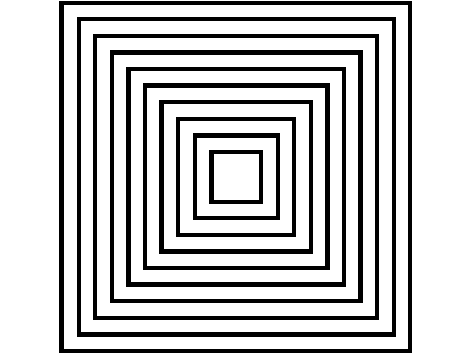
\includegraphics{kultin207}
  \caption{Иллюстрация к задаче 3.}
  \label{fig:kultin207}
\end{minipage}
\end{figure}

\end{document}
